\begin{figure*}
    \centering
    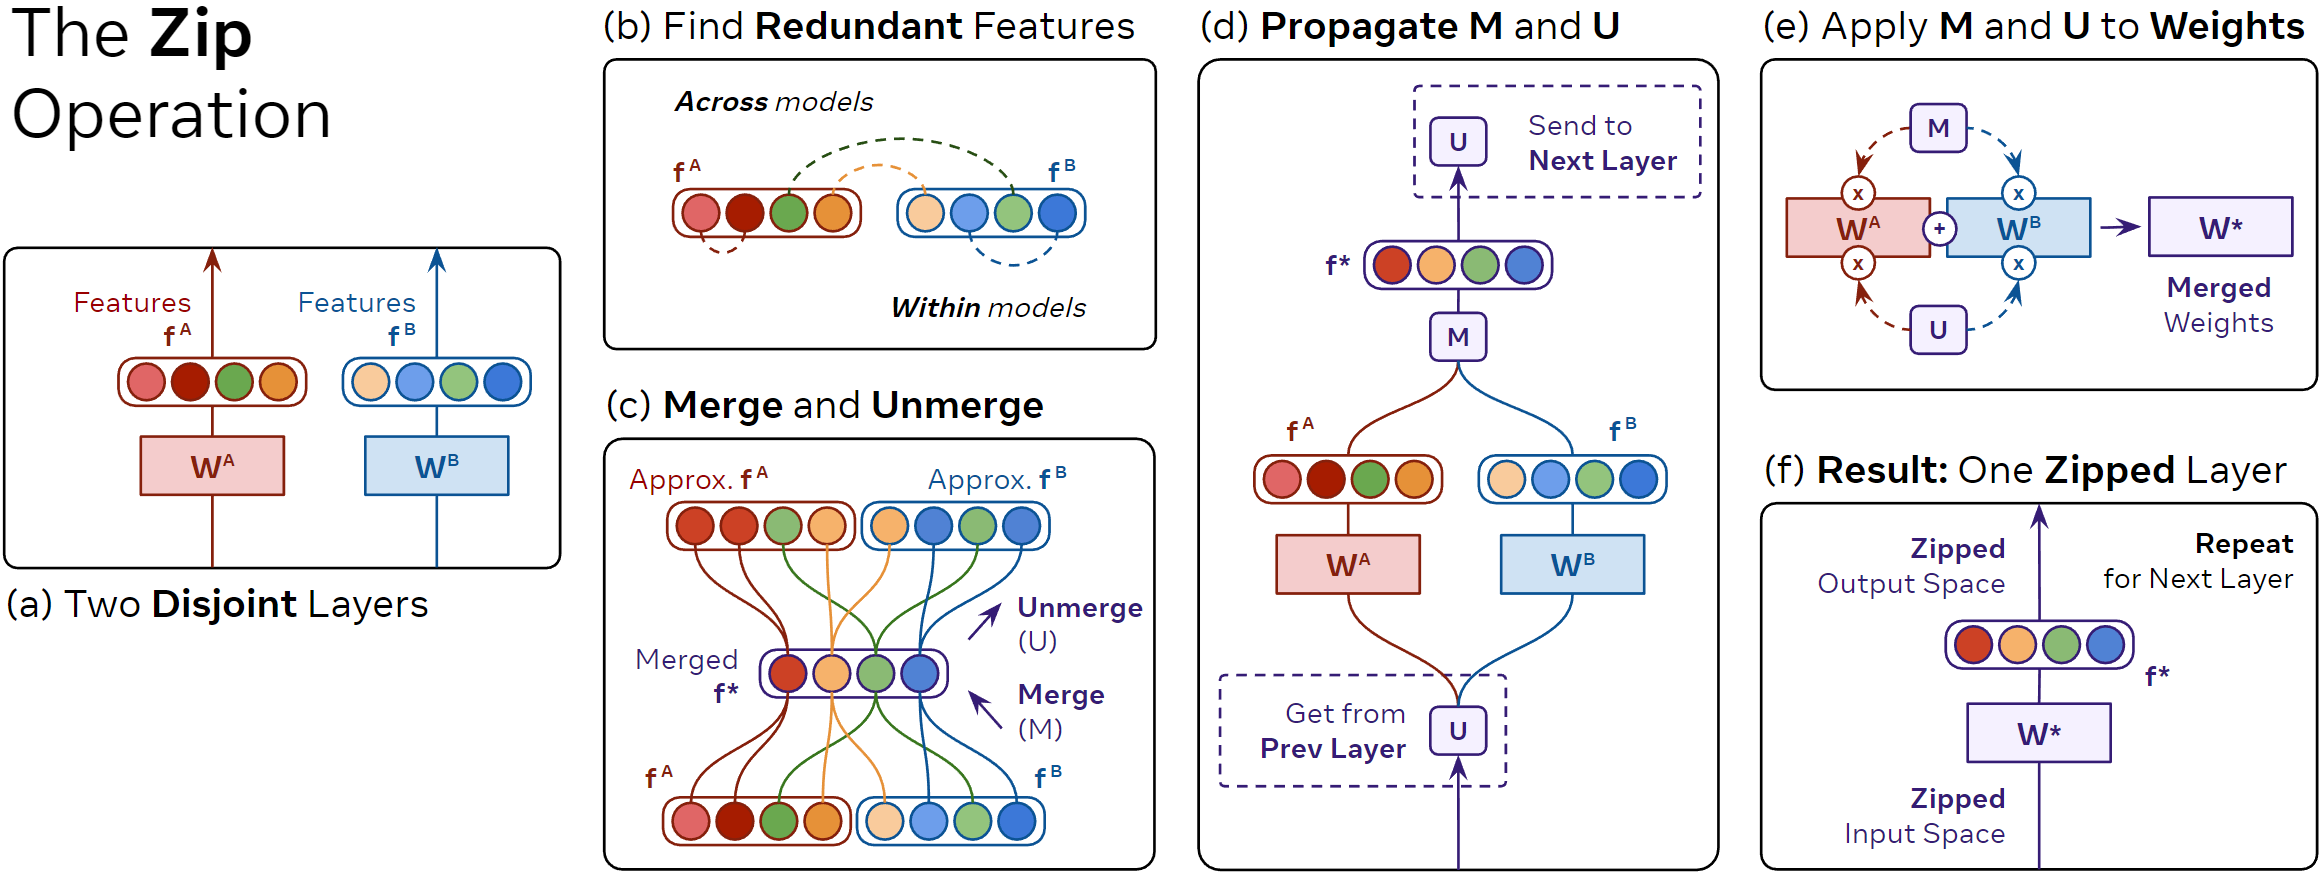
\includegraphics[width=0.95\linewidth]{figures/imgs/zip_it.png}
    \caption{{\bf \name{}} merges models layer-wise by exploiting redundancy in their features. 
    % (a) Starting with completely disjoint layers with weights \modela{$W^{A}$} and \modelb{$W^{B}$} from models trained on different tasks, (b) we match redundant features by comparing their activations \modela{$f^{A}$} and \modelb{$f^{B}$}. (c) We use this matching to produce a merge matrix \modelc{M} to combine \modela{$f^{A}$} and \modelb{$f^{B}$} into a single shared feature space \modelc{$f^{*}$} and a corresponding unmerge matrix \modelc{U} that undoes this operation. (d) In order to align the input space of the next layer, we propagate \modelc{U} forward along network and at the same time receive a \modelc{U} matrix from the previous layer. (e) Once we have both an \modelc{M} for the output, and a \modelc{U} for the input, we can ``zip'' the layers together by applying Eq.~\ref{eq:zip}. (f) The result is a single layer with a shared input and output space, and we can now repeat from (a) on the next layer.
    (a) Output features \modela{$f^{A}$} and \modelb{$f^{B}$} from two disjoint layers are (b) paired with other features based on the similarity of their activations. (c) We produce a merge matrix \modelc{M} to combine the pairs into a single shared output feature space, and a corresponding unmerge matrix \modelc{U} that undoes this operation. (d) We then propagate \modelc{U} up the network to align the next layer's input space, and simultaneously receive the previous layer's \modelc{U} to align our input space. (e) We apply Eq.~\ref{eq:zip} to ``zip'' the layers together using the \modelc{M} for the output and \modelc{U} for the input, producing a single layer (f). We then repeat (a) on the next layer.
    % . (f) We obtain a single layer with a shared input and output space. We then repeat from (a) on the next layer. 
    }
    \label{fig:zip_op}
\end{figure*}